\documentclass[12]{amsart}

\usepackage{amssymb,amsmath}

%\usepackage{refcheck}

\usepackage{graphicx}
\usepackage{amssymb}
\usepackage{mathrsfs}
\usepackage{amsmath}
\usepackage{latexsym}
\usepackage{amssymb}
\usepackage{enumerate}
\usepackage{fullpage} 
\usepackage{setspace}
\usepackage{color}
%\usepackage{ dsfont }
\usepackage{float}
\usepackage{physics}

%new math symbols taking no arguments
\newcommand\0{\mathbf{0}}
\newcommand\CC{\mathbb{C}}
\newcommand\FF{\mathbb{F}}
\newcommand\NN{\mathbb{N}}
\newcommand\QQ{\mathbb{Q}}
\newcommand\RR{\mathbb{R}}
\newcommand\ZZ{\mathbb{Z}}
\newcommand\bb{\mathbf{b}}
\newcommand\kk{\Bbbk}
\newcommand\mm{\mathfrak{m}}
\newcommand\pp{\mathfrak{p}}
\newcommand\xx{\mathbf{x}}
\newcommand\yy{\mathbf{y}}
\newcommand\GL{\mathit{GL}}
\newcommand\into{\hookrightarrow}
\newcommand\nsub{\trianglelefteq}
\newcommand\onto{\twoheadrightarrow}
\newcommand\minus{\smallsetminus}
\newcommand\goesto{\rightsquigarrow}
\newcommand\nsubneq{\vartriangleleft}

%redefined math symbols taking no arguments
\newcommand\<{\langle}
\renewcommand\>{\rangle}
\renewcommand\iff{\Leftrightarrow}
\renewcommand\phi{\varphi}
\renewcommand\implies{\Rightarrow}

%new math symbols taking arguments
\newcommand\ol[1]{{\overline{#1}}}

%redefined math symbols taking arguments
\renewcommand\mod[1]{\ (\mathrm{mod}\ #1)}

%roman font math operators
\DeclareMathOperator\aut{Aut}

%for easy 2 x 2 matrices
\newcommand\twobytwo[1]{\left[\begin{array}{@{}cc@{}}#1\end{array}\right]}

%for easy column vectors of size 2
\newcommand\tworow[1]{\left[\begin{array}{@{}c@{}}#1\end{array}\right]}

\newtheorem{theorem}{Theorem}[section]
\newtheorem{corollary}{Corollary}[theorem]
\newtheorem{lemma}[theorem]{Lemma}
\newtheorem{exercise}[theorem]{Exercise}

\title{Bosonic Codes for Pedestrians}
\author{Faris Sbahi}

\begin{document}
\maketitle

Quantum error correction is necessary to achieve fault tolerant quantum communication. In other words, one must implement a scheme to encode information redundantly into physical degrees of freedom so that information can be preserved in the presence of noise. One such scheme is continuous variable quantum information processing using bosonic modes \cite{braunstein1998error, braunstein2005quantum, niset2008experimentally, aoki2009quantum, lloyd1998analog, lassen2010quantum}. In this case, one encodes information in the space corresponding to the occupation number of a harmonic oscillator. Hence, one can express the code subspace in terms of number states $\{\ket{n}\}^\infty_{n=0}$ \cite{michael2016new}, position and momentum eigenstates $\{\ket{x}\}_{x\in\RR}$ and $\{\ket{p}\}_{p\in\RR}$  \cite{gottesman2001encoding}, or a few coherent states $\{\ket{\alpha}\}_{\alpha\in S}$ (for some finite set $S$) \cite{cochrane1999macroscopically}.

The first studied continuous variable scheme utilizing bosonic modes is known as the two-mode “dual-rail” encoding published in 1995 \cite{chuang1995simple}. Nowadays, there are several bosonic codes being evaluated in the fault tolerant quantum computation race. In this review, we'll consider a few of the most popular contenders: first, we'll develop a practical bosonic error model. Next, we'll study three popular single mode codes with impressive protection capabilities with respect to this model. Then, we'll consider the work of \cite{albert2017performance} to evaluate the performance of these codes and take into account some theoretical considerations. Finally, we'll consider hardware-efficient multi-mode extensions which are notable for their progress toward physical realizability and place these results in the context of the emerging field of bosonic quantum error correcting codes.

\section{Introduction}

\subsection{Definitions}

The generic task of quantum error correction is to find two logical code words---a qubit---embedded in a large Hilbert space. The code words are required to be robust such that if any one of the single, independent errors $E_{l,k} \in \mathcal{E}$ occurs, no quantum information is lost and any quantum superposition of the logical code words can be faithfully recovered. This is equivalent to finding two logical code words $\ket{W_\sigma}$, where $\sigma = \uparrow, \downarrow$, that satisfy the quantum error correction criteria, known also as the Knill-Laflamme conditions \cite{nielsen2002quantum}.

\begin{align}
\label{eq:k-l}
\bra{W_\sigma} E_l^\dag E_k \ket{W_\sigma} = \alpha_{l, k} \delta_{\sigma, \sigma'}	
\end{align}

for all $E_{l,k} \in \mathcal{E}$ such that $\alpha_{l,k}$ are entries of a Hermitian matrix and independent of the logical words. The independence of entries $\alpha_{l,k}$ from the logical code words and the structure of the non-diagonal entries guarantee that the different errors are distinguishable and correctable.

Notationally, we'll refer to a harmonic oscillator's non-Hermitian creation and annihilation operators as $a^\dag$ and $a$, respectively. Furthermore, we define $\hat{n} := \hat{a}^{\dag }\hat{a}$. Recall the relations, with respect to Fock states $\ket{n}$,

\begin{align*}
\hat{a}^{\dagger }|n\rangle &={\sqrt {n+1}}|n+1\rangle, \qquad \hat{a}\ket{n}={\sqrt {n}}|n-1\rangle \\
\hat{n}\ket{n} &= n\ket{n} \\
[\hat{a}, \hat{a}^{\dag }]&=1, \qquad[\hat{n},\hat{a}^{\dag }]=\hat{a}^{\dag }, \qquad[\hat{n}, \hat{a}]=-\hat{a},
\end{align*}

Note the natural convention of calling $\hat{n}$ the "number" operator, based upon its Fock state relation above. Hence, we can develop a notion of parity by considering action by

\begin{align}
\label{eq:parity}
(-1)^{\hat{n}}	
\end{align}


Also, recall the definition of coherent states $\ket{\alpha}$ which refer to eigenstates of the annihilation operator,

$$
|\alpha\rangle =e^{-{|\alpha|^2\over2}}\sum_{n=0}^{\infty}{\alpha^n\over\sqrt{n!}}|n\rangle =e^{-{|\alpha|^2\over2}}e^{\alpha\hat a^\dagger}|0\rangle ~,
$$

We will call errors generated by action of $\hat{a}$ "loss" errors, by $\hat{a}^\dag$ "gain" errors, and by $\hat{n}$ "dephasing" errors. 

\section{Bosonic Error Models}

It's especially important to consider a practical bosonic error model before designing a bosonic code because of the unique nature of photon errors. In particular, photons are prone to loss, and photon-photon interactions are extremely weak. Hence, bosonic QEC codes focus on correcting photon-loss errors using very limited forms of photon-photon interactions while striving to be hardware efficient \cite{niu2018hardware}. 

We can describe this using the pure-loss channel, which is a model for broadband-line and free-space communication and it is the most common incoherent error pro- cess in optical and microwave cavities \cite{albert2017performance}. The second most common error is cavity dephasing, which is caused by fluctuations in the cavity frequency. Optical cavities have to be actively stabilized to fix the frequency, but the effects of such fluctuations are small relative to effects of energy loss, particularly in microwave cavities. 

The bosonic pure-loss channel is given by $N_\gamma = \exp(\kappa t D)$ ($\gamma$ defined below) with Lindblad superoperator $D(\cdot) = \hat{a} \hat{a}^\dag - 1/2 \{ \hat{n} , \cdot \}$, excitation loss rate $\kappa$,  and time interval $t$ \cite{albert2017performance}. Another way to represent this is in the Kraus representation with Kraus operators

\begin{align}
\label{eq:kraus}
E_l &= \Big(\frac{\gamma}{1-\gamma}\Big)^{l / 2} \frac{\hat{a}^l}{\sqrt{l!}}(1 - \gamma)^{\hat{n} / 2}
\end{align}
where
$$
\gamma = 1 - \exp(- \kappa t)
$$

This is derived by integrating over all the possible photon loss "jump" times of exactly $l$ photon jumps during a small finite time interval $\delta t$ \cite{chuang1997bosonic}, similar in spirit to the Feynmann path integral. Therefore, the channel can be described as 

$$
N_\gamma = \sum_l^\infty E_l \rho E_l^\dag
$$

for density operator $\rho$.

Observe that this channel does not contain the identity as a Kraus operator when $\gamma \neq 0$ due to the "no-jump" (also "damping" or "back-action") term $(1-\gamma)^{n / 2}$ which results from the non-triviality of observing no photon jump. So, even if there is no loss, there is still redistribution of the probabilities of being in Fock states. Furthermore, both this redistribution and photon loss take place over continuous time and so continuous time evolutions results in an infinite set of possible errors. Therefore, the error correction criteria (\ref{eq:k-l}) can't be utilized directly. 

Instead, one can expand each error operator in powers of $\kappa \delta t$ (where again $\delta t$ is a small finite time interval) and choose to correct up to a given highest order. This is termed "approximate quantum error correction" \cite{mandayam2012towards}. It is then enough to satisfy the quantum error correction criteria (\ref{eq:k-l}) only approximately such that the original state can be recovered with an accuracy given by the same highest order in $\kappa \delta t$ \cite{michael2016new}.

So, if we perform a Taylor series expansion of each of the Kraus operators $E_l$ above and consider correcting both the photon loss and back-action contributions up to order $O[(\kappa \delta t)^L]$ for some specified $L$, then we can derive a new set of approximate error correction conditions. The full derivation is contained in \cite{michael2016new} but we summarize the results below which we'll utilize in our analysis in the next sections.

First, observe that Kraus operators $E_{l>L}$ can be ignored since they have the effect of order at least $L+1$. So, denote $E_{\mu, l}$ as the $\mu$th entry of the expansion of (\ref{eq:kraus}) in powers of $(\kappa\delta t)^{1/2}$. Now, for convenience sake, expand each Kraus operator $E_{l \leq L}$ into two contributions

\begin{align*}
E_l &= B_l + C_l + O[(\kappa \delta t)^{L + 1/2}]	\\
\intertext{where}
B_l &= \sum_{\mu = l }^L E_{\mu, l}(\kappa \delta t)^{\mu / 2} \\
C_l &= \sum_{\mu = L+1 }^{2L - 1} E_{\mu, l}(\kappa \delta t)^{\mu / 2} \\
\end{align*}

Then, we can rewrite our channel as 

\begin{align*}
N_\gamma &= \sum_{l=0}^\infty E_l \rho E_l^\dag\\
&= \sum_{l=0}^L E_l \rho E_l^\dag + O[(\kappa \delta t)^{L + 1}] \\
&= \sum_{l=0}^L(B_l \rho B_l^\dag + B_l \rho C_l^\dag + C_l \rho B_l^\dag) + O[(\kappa \delta t)^{L + 1}]
\end{align*}

Hence, one can ignore the negligible $O[(\kappa \delta t)^{L + 1}]$ part of the interference terms and verify only that the effect of the remaining important part is independent of the logical code words. Together, if the error operators $B_l$ and $C_l$ for all $0 \leq l \leq L$ satisfy the two following conditions,

\begin{align}
\label{eq:aqec}
\begin{split}
\bra{W_\sigma} B_l^\dag B_l \ket{W_{\sigma'}} &= \beta_l \delta_{\sigma \sigma'} \\
\bra{W_\sigma} B_l^\dag C_l \ket{W_{ \sigma'}} &= \nu_l \delta_{\sigma \sigma'}	+ O[(\kappa \delta t)^{L + 1}]
\end{split}
\end{align}

then the original state can be corrected up to order $O[(\kappa \delta t)^L]$.

These equations have the interpretation of allowing us to determine to what order a code corrects both loss errors and back-action errors. In this case of binomial codes, we'll see that we can correct back-action to the same order as photon loss. Other codes have addressed the back-action contribution by constructing multimode codes \cite{chuang1997bosonic}. These codes avoid no-jump evolution by combining two or more physical elements with identical decay rates and constructing the logical code words such that they are superpositions of states with the same combined total excitation number.

\section{Single Mode Codes}

First, we emphasize why we must establish new codes for bosonic systems in the first place. Perhaps, we can instead use a simple encoding of $M$ qubits: $2^M$ Fock states cover photon numbers $0, 1, . . . , (2^{M - 1})$. Hence, we can simply use a Fock state's binary representation, $\ket{n} = \ket{b_{M-1} b_{M-2} \cdots b_0 }$. Then, we can allow the $j$th binary digit represents the eigenvalue $(1 + Z_j)/2$ for the corresponding physical qubit. For example, for Fock state $n=16$: $\ket{10000}$. However, now consider if photon loss occurs (which we've noted to be frequent): $\hat{a}\ket{10000} \mapsto \ket{01111}$--$\hat{a}$ generates 4 correlated errors. Hence, as the authors of \cite{michael2016new} note, QEC schemes based on models of independent single qubit errors cannot be easily transferred to this problem. Luckily, the stabilizer formalism provides useful intuition for codes we'll discuss (see Section \ref{sec:multi-binom}).

\subsection{A Simple Example}
\label{sec:simple}

So, consider a simple bosonic code to protect against $\mathcal{E} = \{ I, \hat{a} \}$. Define 

$$
\ket{W_\uparrow} = \frac{\ket{0} + \ket{4}}{2}\\
\ket{W_\downarrow} = \ket{2}
$$. Hence, $\ket{E_1} = \ket{3}$ and $\ket{E_2} = \ket{1}$ give our error words. 

As it turns out, we have the capability of very high fidelity quantum non-demolition measurements of the photon number parity \cite{sun2014tracking}. Hence, we can efficiently distinguish these logical/error words by measuring photon number and checking modulo 2. If the syndrome is 0, then we assume no error has occurred. If the syndrome is 1, we can perform a unitary operation swapping $\ket{E_1}$ with $\ket{W_\uparrow}$ and $\ket{E_2}$ with $\ket{W_\downarrow}$.

Furthermore, observe that both logical states have the same mean photon number i.e. $\bra{W_\sigma} \hat{n} \ket{W_\sigma} = 2, \forall \sigma$. Therefore, $\hat{a} : \alpha\ket{W_\uparrow} + \beta\ket{W_\downarrow} \mapsto \alpha \ket{E_1} + \beta \ket{E_2}$. We say that this condition implies that there is no "deformation".

So, how can we generalize from here? Well, we can add greater spacing between states so that we can detect higher order loss errors or alternatively gain errors. Intuitively, if there was a greater separation in photon number of the Fock states that define $\ket{W_\sigma}$ then one could measure modulo the spacing ("generalized parity") and determine how many loss events took place. For example, if we considered

$$
\ket{W_\uparrow} = \frac{\ket{0} + \sqrt{3}\ket{6}}{2}\\
\ket{W_\downarrow} = \frac{\ket{3} + \sqrt{3}\ket{9}}{2}
$$

and measured the photon number modulo 3, then we'd say that syndrome 0 indicates no error, syndrome 1 indicates a single loss, and syndrome indicates double loss.

 Furthermore, observe that action by $n$ "dephases" in the sense that, after transformation, the relative phases of the Fock states are transformed. This action leads to a superposition of codewords and error words. We can detect this dephasing error by making projective measurement onto the logical codeword basis and if the measurement eigenvalue is negative and no photon loss is detected, then we can perform the unitary state transfer $\ket{E_\sigma} \leftrightarrow \ket{W_\sigma}$ as prescribed above.
 
\subsection{Cat Codes}

Cat codes were first discovered in \cite{cochrane1999macroscopically} in the case of a single mode. Several papers have extended these codes to the multi-mode case in order to correct more errors or offer a hardware-efficient implementation \cite{albert2018multimode, leghtas2013hardware, mirrahimi2014dynamically} and we will summarize these results in Section \ref{sec:multi-cat}. We mirror the treatment of \cite{mirrahimi2014dynamically} since their four-photon driven dissipative process suppresses bit-flip errors.

Now, consider using a superposition of "well-separated" coherent states as the logical state encoding. Usually, cat codes are presented in the case of correcting a single loss error $\hat{a}$, but it can be generalized to the multiple-loss case \cite{albert2018multimode}. Nevertheless, we'll present the single-loss case.

It is aesthetically pleasing to develop the code in terms of symmetries over a stabilizing operator $J \sim \hat{a}^4$. In other words, our logical code space, where each element is a superposition of coherent states, is preserved under action by $J$ (up to a phase), similarly to the familiar stabilizer formalism.

We observe that parity, as defined in (\ref{eq:parity}), commutes with $J$. Hence, we can use parity to label basis states of our code subspace by defining parity operator

\begin{align*}
P_{\Pi} = \frac{1+(-1)^{\hat{n}}}{2}	
\end{align*}

where $\Pi \in \{0, 1\}$.

We claimed that logical cat states are well-separated and elaborate this notion to mean, in particular, that the basis elements of cat states are projections of the parity operator on coherent states. Hence,

\begin{align*}
\ket{\alpha_\Pi} &= N_\Pi P_\Pi \ket{\alpha}
\end{align*}

where $N_\Pi$ is the normalization factor. Hence, we observe that

\begin{align*}
\ket{\alpha_\Pi} \sim \begin{cases} \ket{\Pi},  &\alpha \rightarrow 0\\ \ket{\alpha} + (-1)^\Pi \ket{-\alpha}, &\alpha \rightarrow \infty \end{cases}
\end{align*}

So, observe the following relations

\begin{align}
\label{eq:cat-rels}
\begin{split}
\hat{a} \ket{\alpha_0} &= \ket{\alpha} - \ket{-\alpha} = \ket{\alpha_1} \\
\hat{a} \ket{\alpha_1} &= \ket{\alpha} + \ket{-\alpha} = \ket{\alpha_0} \\
\hat{a} \ket{i\alpha_0} &= i(\ket{i\alpha} - \ket{-i\alpha})\\
\hat{a} \ket{i\alpha_1} &= i(\ket{i\alpha}  + \ket{-i\alpha})
\end{split}
\end{align}

which we will utilize shortly. So, we can define logical code states $C_\mu, \mu \in \{ \uparrow, \downarrow \}$ as 

\begin{align*}
\ket{C_\mu^{\alpha, \Pi}} &= N_{\mu, \Pi} (\ket{\alpha_\Pi} + (-1)^\mu \ket{i \alpha_\Pi})\\
&= N_{\mu, \Pi} \sum_{p\text{ even/odd}}^{[0, \infty)}\sqrt{\exp(-|\alpha|^2)\frac{
\alpha^{4p}}{2p!}}\ket{2p}
\end{align*}

where $N_{\mu, \Pi}$ are the normalization factors which evidently become equal as $\alpha \rightarrow \infty$. 


We can show that there is a $\mu$-dependence in the normalization factor which is suppressed exponentially in $\alpha^2$ \cite{albert2018multimode}. Similarly, it turns out that that when considering $p$th order dephasing errors $\hat{n}^p$, the term

$$
\bra{C^{\alpha, \Pi}_{\uparrow}} n^p \ket{C^{\alpha, \Pi}_{\uparrow}} - \bra{C^{\alpha, \Pi}_{\downarrow}} n^p \ket{C^{\alpha, \Pi}_{\downarrow}}
$$ 

is nonzero by virtue of the $\mu$-dependence of the normalization factors. Hence, similarly, this difference goes to zero as $\alpha \rightarrow \infty$. So, according to (\ref{eq:k-l}), cat states are potentially immune from any order of dephasing.

\subsubsection{Discrete Loss Errors}

Now, we use the relations above (\ref{eq:cat-rels}) to specify action of $\hat{a}$ on our cat code states.

\begin{align*}
\hat{a}	\ket{C^{\alpha, 0}_{\uparrow}} &= \hat{a}	\ket{C^{\alpha, 1}_{\downarrow}}, \qquad
\hat{a}	\ket{C^{\alpha, 0}_{\downarrow}} = \hat{a}	\ket{C^{\alpha, 1}_{\uparrow}}\\
\hat{a}	\ket{C^{\alpha, 1}_{\uparrow}} &= \hat{a}	\ket{C^{\alpha, 0}_{\uparrow}},\qquad 
\hat{a}	\ket{C^{\alpha, 1}_{\uparrow}} = \hat{a}	\ket{C^{\alpha, 0}_{\uparrow}}
\end{align*}

Hence, we see that application of $\hat{a}$ on an even parity ($\Pi = 0$) cat state transforms to the odd parity subspace ($\Pi = 1$) while also creating a logical bit flip ($\uparrow \leftrightarrow \downarrow$). On the other hand, $\hat{a}$ transforms an odd parity state to an even parity state without the logical bit flip. Therefore, to the order that the approximate quantum error conditions (\ref{eq:aqec}) are satisfied, the quantum information is preserved and, as long as photon jumps are detected and recorded, there is no further correction needed. In other words, the limiting factor of the accuracy of cat codes is independent of action of detected single-loss $\hat{a}$.

However, if $\hat{a}^2$ is applied, then we evidently generate a logical bit flip while preserving parity. Therefore, our parity measurement will indicate no change in parity despite a non-trivial transformation taking place. Hence, $\hat{a}^2$ is non-correctable.

\subsubsection{Dephasing Errors}
\label{sec:cat-deph}

As noted above, dephasing errors are suppressed to the same order that the normalization constants for the $p$th moment of photon number are equivalent for each of the logical states. In particular, dephasing errors are suppressed exponentially in $\alpha^2$.

\subsubsection{Continuous Errors}

Now, we can use the approximate quantum error correction conditions we developed in the previous section. Observe that from equation (\ref{eq:kraus}), $E_1 = \Big(\frac{\gamma}{1-\gamma}\Big)^{1 / 2} \hat{a} (1 - \gamma)^{\hat{n} / 2} = \hat{a} \gamma^{1/2} (1- \gamma)^{\hat{n}}$. Hence, for all $\Pi$,

\begin{align*}
&\bra{C^{\alpha, \Pi}_{\uparrow}}E_1E_1^\dag\ket{C^{\alpha, \Pi}_{\uparrow}} - \bra{C^{\alpha, \Pi}_{\downarrow}}	E_1E_1^\dag\ket{C^{\alpha, \Pi}_{\downarrow}}	\\
&\approx \kappa\delta t (\bra{C^{\alpha, \Pi}_{\uparrow}}\hat{n}\ket{C^{\alpha, \Pi}_{\uparrow}} - \bra{C^{\alpha, \Pi}_{\downarrow}}	\hat{n}\ket{C^{\alpha, \Pi}_{\downarrow}}\\
&\approx 4 \kappa \delta t |\alpha|^2  \exp(-|\alpha|^2)(\sin |\alpha|^2 + \cos|\alpha|^2)
\end{align*}

and so the approximation quantum error correction conditions (\ref{eq:aqec}) are violated when this is nonzero, since there exists uncorrectable errors of order $O(\kappa \delta t)$ and we are consider single-loss errors. Observe that the term goes to zero as $\alpha\rightarrow \infty$, however. This is expected since this is the first moment of photon number analyzed in Section \ref{sec:cat-deph}. Hence, to suppress these errors, we may require a large $\alpha$. Recalling that the $\alpha$ label for a coherent state $\ket{\alpha}$ indicates the mean photon number for the Poissonian distribution of number states, we see that this potential increase in average photon number relative to other codes can then introduces a greater error rate.

\subsection{Binomial Codes}

Now, we consider a new class of codes known as "binomial codes" which were developed in  \cite{michael2016new}. Binomial codes are similar in spirit to the code we described in Section \ref{sec:simple}, since we use Fock states as our physical degrees of freedom to encode logical states.


So, consider if we desire to protect against $\mathcal{E} = \{I, a, a^2, \cdots, a^L, a^\dag, \cdots, (a^\dag)^G, N, \cdots, N^D \}$. The authors then suggest a simple class of codes of the following form

$$
\ket{W_{\uparrow / \downarrow}} = \frac{1}{\sqrt{2^N}} \sum_{ p\text{ even/odd}}^{[0, N+1]} \sqrt{\binom{N+1}{ p }} \ket{p(S+1)}
$$

with spacing $S = L+G$ and maximum order $N = \max\{L, G, 2D\}$. Hence, we can see that the spacing between Fock states is given by $S+1$ and so we can distinguish errors by measuring photon number modulo $S+1$. Again, this works as a result of the spacing since a state can be shifted downward by repeated application of $\hat{a}$ up to $S$ times until becoming equivalent to the next Fock state originally below.

\subsubsection{Discrete Loss/Gain Errors}

 Furthermore, they consider loss errors in the context of the discrete error correction conditions (\ref{eq:k-l}) and show that

$$
\bra{W_\uparrow}(\hat{a}^\dag)^l\hat{a}^l \ket{W_{\uparrow}} = \bra{W_\downarrow}(\hat{a}^\dag)^l\hat{a}^l \ket{W_{\downarrow}}
$$ 

for $l \leq \max\{L, G\}$. They show this by observing that $(\hat{a}^\dag)^l\hat{a}^l = \hat{n}^l$. Then, they write the difference in the $l$th moment of photon number of codewords as the $l$th derivative of $(1+x)^{N+1}\vert_{x=-1}$ with $l \leq \max\{L, G\}$ (up to a factor) by using the binomial formula. Furthermore, since we're using orthonormal Fock states as our basis it's clear that

$$
\bra{W_\sigma}(\hat{a}^\dag)^l\hat{a}^m \ket{W_{\sigma'}} = 0
$$  

for $l, m \leq \max\{L, G\}, l \neq m$. So, the discrete error correction conditions are obeyed.

Hence, since we show that the $l$th moment of $\ket{n}$ is equivalent for both logical code words, it also follows that the mean photon number is equivalent for both code words given that the mean is the first moment. So, there is no deformation by measuring the mean photon number.

Observe that from above the "quantum error correction matrix" as defined by the matrix elements $Q_{(l, k)} = \alpha_{l, k}$ from (\ref{eq:k-l}) is diagonal when only considering loss/gain errors.

\subsubsection{Discrete Dephasing Errors}

Now, if we consider dephasing errors as well, the error correction matrix is no longer necessarily diagonal but is still Hermitian (as required). For that reason, to detect and recover those errors one needs to make projective measurements in an orthonormalized basis, as with the code in Section \ref{sec:simple}. After a detection of an error, the original state is recovered by a unitary operation performing a state transfer between the subspaces of the error and logical code words.

\subsubsection{Continuous Errors}

Refer back to the approximate quantum error conditions (\ref{eq:aqec}). Both $B_l^\dag B_l$ and $B_l^\dag C_l$ up to accuracy of $(\kappa \delta t)^L$ can be written as a polynomial of $\hat{n}$ with the highest degree of $L$ \cite{michael2016new}. From above, the binomial code words protected against $L$ photon losses have equal expectation value of $hat{n}^l$, for all $l \leq L$ and for both of the code words, which implies that approximate quantum error conditions are satisfied for them.

Observe, however, that this is a theoretical bound on a recovery process when employing this code It remains to identify a specific, tractable process within this threshold. Indeed, the authors show that the simple process of checking parity and applying the appropriate unitary to swap error words and logical code words suffices.
\subsection{GKP Codes}

While all codes discussed so far are defined using a dis- crete (i.e., countable) basis, the Gottesman, Kitaev, and Preskill (GKP) codes [13] are defined using the continu- ous basis of non-normalizable eigenstates of the position operator xˆ. A unique resulting feature of GKP codes is that the correctable errors themselves form a continuous set. The simplest ideal qubit GKP words are

\begin{align*}
\ket{GKP_{\uparrow/\downarrow}} \sim \sum_{p\text{ even/odd}}^{(-\infty, \infty)} \hat{D}\Big(p \sqrt{\frac{\pi}{2}} \Big) \ket{\hat{x} = 0} 	
\end{align*}


  where $\hat{D}$ is the displacement operator from Eq. (10) and $\ket{\hat{x} = 0}$ is the starting position eigenstate. In position space, such states are infinite combs of position eigenstates spaced $2\sqrt{\pi}$ apart, so the effective spacing between the two logical states is $S=\sqrt{\pi}$. The same result holds in momentum ($\hat{p}$) space via Fourier transform of Eq.(36). Naturally, all position and momentum shifts $\exp(-iu\hat{p})\exp(-iv\hat{x})$ with $|u|, |v| \leq \sqrt{\pi}/2$ are correctable. However, the GKP codes can also correct any error operators expandable in the basis of correctable shifts. Careful expansion of photon loss $\ket{a}$ and other errors [20] has confirmed that GKP codes can in principle (i.e., for small enough $\kappa \delta t$) correct photon loss, gain, and dephasing errors.
  
The ideal GKP code words (36) contain both an infinite number of photons and states which are perfectly squeezed in the $\hat{x}$ quadrature. To make the codes experimentally realizable, the superposition in Eq. (10) has to be filtered (to keep the photon number finite) and a distribution of states has to be substituted for the sharp $\ket{\hat{x}=0}$ state (to account for imperfect squeezing). In the traditional form of the approximate codes, a $p$-dependent Gaussian filter is put into the sum in Eq. (36) and a Gaussian wavepacket is substituted for $\ket{\hat{x}=0}$. However, the choice of filter and starting state can be arbitrary. There are a handful of theoretical proposals [98–100] (see also Ref. [101] for an error analysis of GKP states), including one based on a clever use of phase estimation [20], to realize such approximate GKP states. GKP states are also useful in designing highly precise gates for other quantum computing architectures [102].

The approximate code words are not perfectly orthogonal, so one must take into account the error coming from the non-orthogonality. Since the ideal GKP states have in- finite photon number, the approximate GKP states must contain a sufficiently high number of photons in order to manage such imperfections. An optimistic [20] estimate for this photon number is $\bar{n} = 4$, which uses the traditional form of the approximate code words and bounds the error probability coming from the non-orthogonality at about 1\% (Eq. (38) of Ref. [13]). Using the same approximate code words, a photon number of 2 implies a 9\% error bound. As a result, the traditional form of the approximate code words is expected to contain more photons than, e.g., the smallest ($\bar{n} = 2$) binomial code (2).

However, the GKP code words can protect against a larger set of errors than the minimal binomial code. Due to the various choices of starting state and filter as well as due to the difficulty of comparing continuous correctable error sets to discrete ones, a detailed comparison of the relative capabilities of the GKP and binomial/cat classes of codes remains to be done.

\section{Discussion}

\subsection{Theoretical Comparisons}

The single-mode binomial codes require an explicit correction gate at every timestep whether or not a photon jump has occurred. However, binomial codes satisfy the approximate quantum error correction conditions to order $\delta t$ with a smaller average photon number: $\bar{n} = 2$ for the code of Eq. (2), rather than $\bar{n} = 2.3$ for the cat code that minimizes Eq. (32). Furthermore, the binomial codes operate in a restricted Hilbert space, which could be beneficial for the practical construction of the unitary operators required for error diagnosis and recovery. This particularly applies to errors involving $\hat{a}^\dag$ operators, whose operation on cat codes is less straightforward than $\hat{a}$ operators alone.

The Fock state distributions of the binomial and cat codes are binomial and Poissonian, respectively. As the average number of photons is increased (larger N), both of these distributions approach a normal distribution, and so the binomial and cat codes asymptotically approach each other. 

% TODO
Furthermore, since no-jump evolution damps coherent states, $(1 - \gamma)^{\hat{n}}\ket{\alpha} = \ket{(1 - \gamma) \alpha}(1 - \gamma)^{\hat{n}}\ket{\alpha} = \ket{(1 - \gamma) \alpha}$, the only necessary correction is a “re-pumping” of the cat states. This can be achieved using a discrete unitary correction operation (analogous to the binomial codes) or continuous non-linear amplification coming from an engineered reservoir [17, 18] (analogous to similar passive/autonomous error correction schemes [94, 95]). The basic principle of passive schemes is stabilization of a manifold of codewords as an attractive (stable) fixed-point of drives and dissipation so that the only remaining task is to track generalized parity for photon jumps [18]. The cat codes based on equal amplitude coherent state superpositions, cf. Eq. (31), are ‘natural’ candidates for these purposes since they require only gradual continuous inversion of the damping of the coherent state amplitude without active discrete correction stages. The two-leg cat has already been stabilized by reservoir engineering to achieve dominant two-photon drive and two-photon dissipation [96].

\begin{figure}
\centering
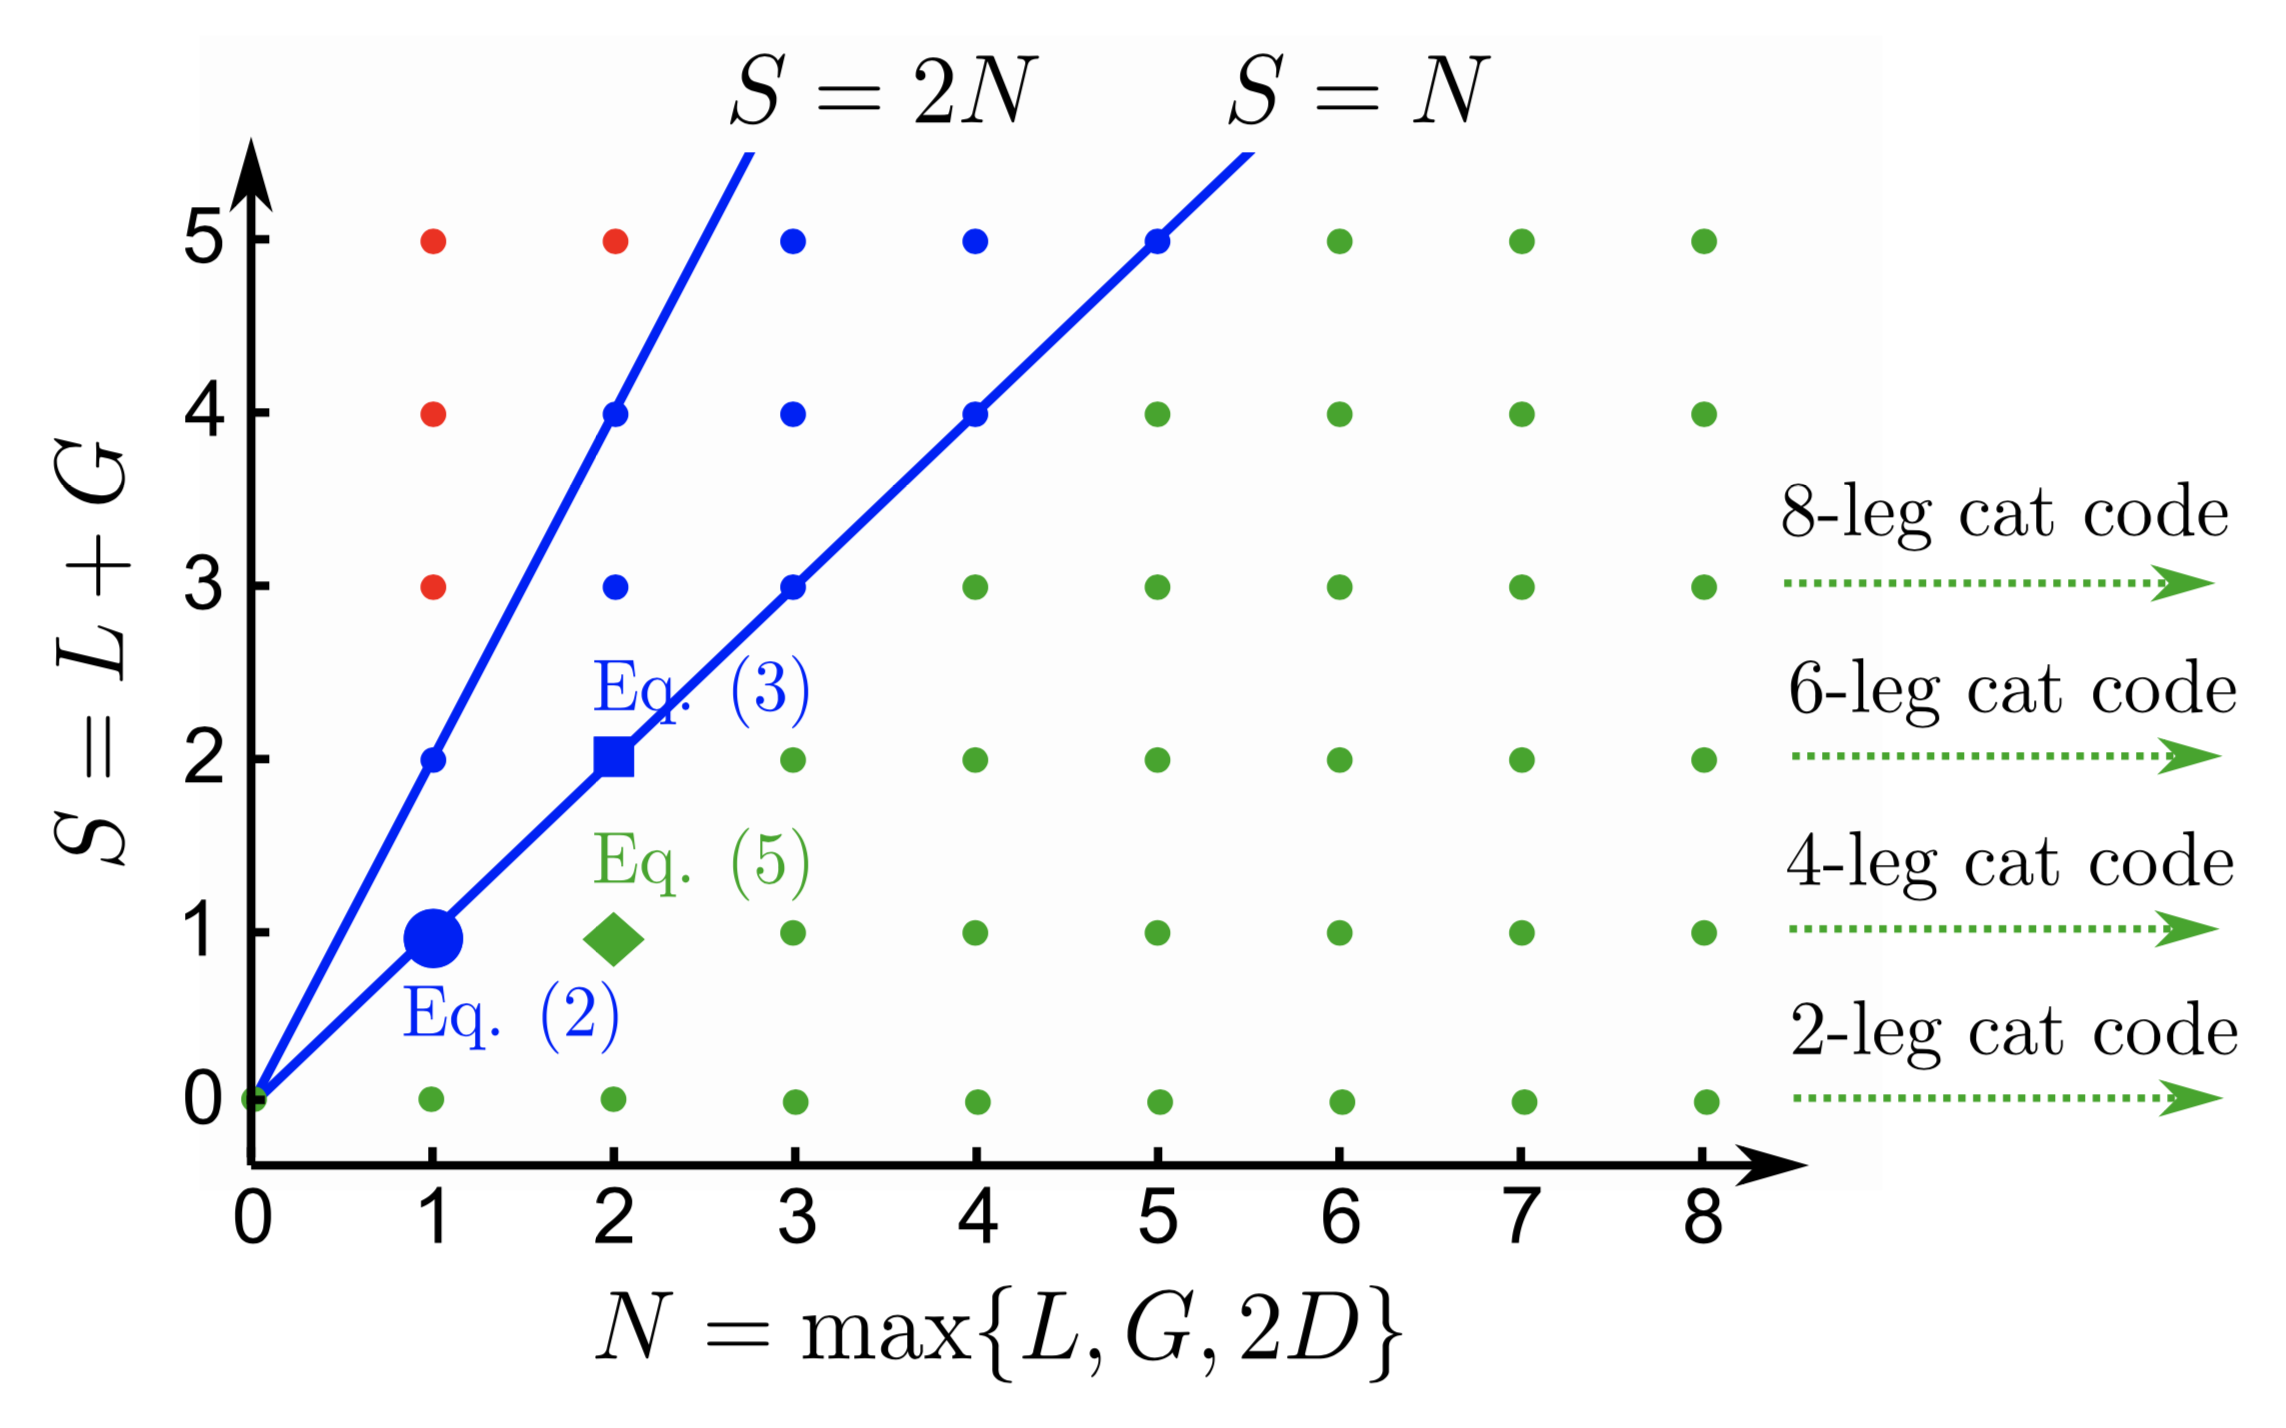
\includegraphics[width=0.5\linewidth,keepaspectratio]{binom_cat.png}	
\caption{Figure borrowed from \cite{michael2016new} comparing binomial codes to cat codes. Observe that, in principle, unlimited dephasing errors can be tolerated by cat codes.}
\end{figure}

\subsection{Performance Comparisons}

VV Albert considers "channel fidelity", $F_\mathcal{E}$, which is the overlap between the initial state and the final state when considering an initial Bell state such that only the first qubit is acted on by the channel

Optimal recovery for each code is computable via a semi-definite program

\begin{figure}[H]
\centering
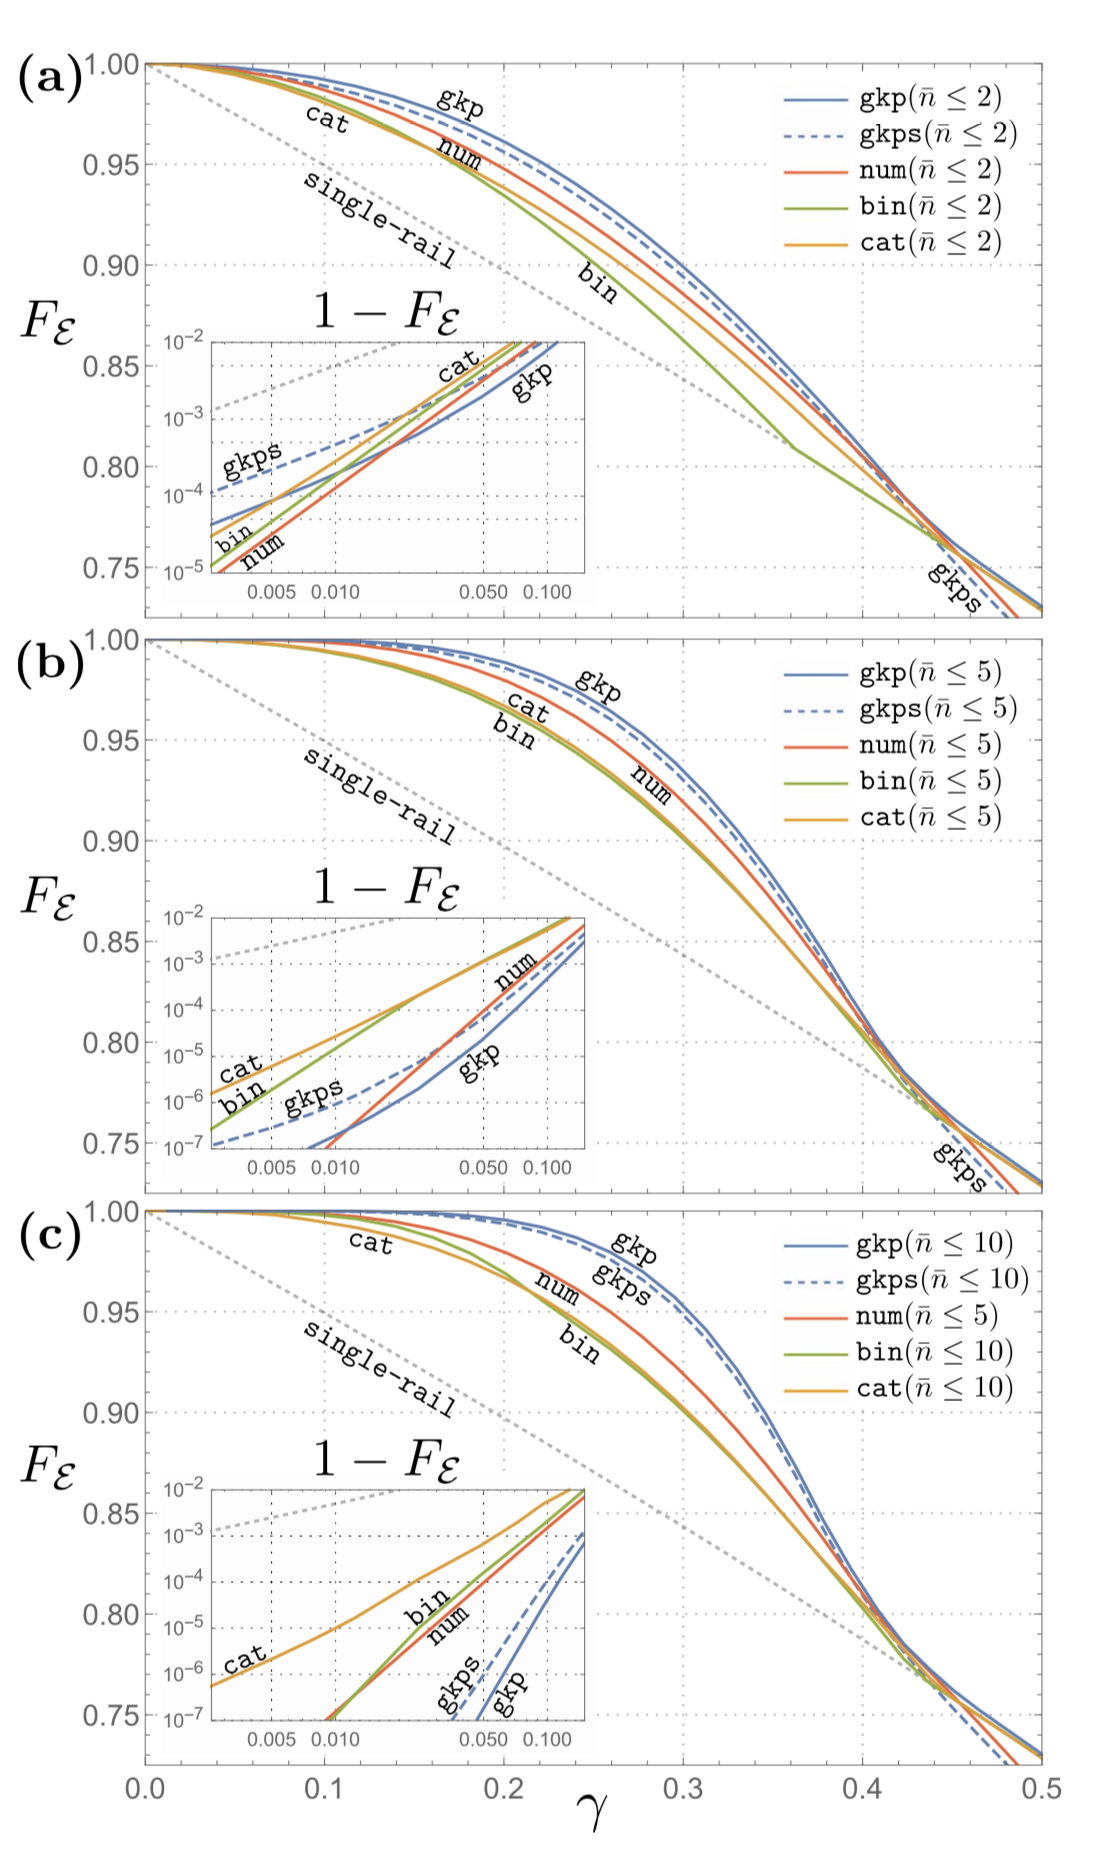
\includegraphics[width=0.5\linewidth,keepaspectratio]{fidelity.png}	
\end{figure}

In this paper \cite{noh2018improved}, we prove that the GKP codes achieve quantum capacity of Gaussian loss channels up to at most a constant gap from an upper bound of the quantum capacity. In section II, we review and summarize key properties of Gaussian loss, amplification and random displacement channels, which will be used in later sections. In section III, we provide an im- proved upper bound of quantum capacity of the Gaussian loss channel, both in energy-constrained and unconstrained cases by introducing a slight modification of an earlier result in [18] (Theorems 10, 11 and 12; see also Eq.(42) for an improved upper bound of Gaussian random displacement channel ca- pacity). In section IV, we discuss experimental implementa- tion of the GKP codes and prove that the achievable quan- tum communication rate with the GKP codes deviates only by a constant number of qubits per channel use from our im- proved upper bound, assuming an energy-unconstrained sce- nario (Theorem 14). In section V, we address the energy- constrained encoding scenario and formulate a biconvex opti- mization problem to find an optimal set of encoding and de- coding which maximize the entanglement fidelity. We solve the biconvex optimization using alternating semidefinite pro- gramming (SDP), and show that the GKP code emerges as an optimal solution.
\subsection{Multi-Mode Extensions}

Here we briefly summarize recent results based upon these fundamental single-mode codes with the intention of creating near-term physically realizable codes with similar or improved error-correction capabilities.

\subsubsection{Cat Codes}\label{sec:multi-cat}

In this work, we introduce a complete error-correction method for the two-mode scheme II. A side-by-side com- parison to scheme I is in Table I. The leading uncor- rectable errors for both schemes are of the same order, a2 for scheme I and ab for scheme II, so the code subspaces in both schemes are of comparable quality. However, while retaining all of the benefits of the cat codes, scheme II enjoys several advantages, including most importantly a drastic reduction of the order of the nonlinearity required for realization. Three- and higher-mode extensions of scheme II further increase the error-correcting properties of the codes, e.g., an M-mode code for M ≥ 2 enjoys a leading-order uncorrectable loss error of a1 a2 · · · aM . We summarize these advantages below.

One can show that a dominant dissipative term $\kappa_\# D_\#$ (1.3) is able to continuously suppress (or, in the sense of Ref. [43], passively protect from) any dephasing error processes without the need for error syndrome measure- ment and recovery operations. In this work, we refer to an error-correction process that is continuous in time and that does not require active measurement and feed- back operations as continuous quantum error correction (QEC) [24, 44–52].1 Both schemes also admit discrete QEC (i.e., conventional protection via non-demolition measurements of error syndromes and adaptive control) against photon loss, but only scheme II can perform both QEC processes simultaneously using currently available techniques.

The scheme I syndrome is the photon number parity,

Πˆ = (−1)nˆ , (1.4)

and parity measurements [54] and full-blown discrete QEC [32] for scheme I have been implemented using cur- rent superconducting circuit technologies. Separately, continuous QEC against dephasing has been achieved for the simplest cat-code with jump operator a2 − α2 [31] (such a cat code cannot protect from photon loss). However, it is impossible to perform both discrete and continuous QEC for scheme I simultaneously with cur- rent technologies. The established measurement tech- nique implements an entangling gate eiHt generated by the naturally occurring cross-Kerr interaction H = χnˆσz (where σz acts on an ancillary junction). The dissipa- tor FI commutes with eiHt only at t = π/χ and not at any other intermediate time. Therefore, the protective dissipation due to FI has to be turned off during the measurement.

The scheme II syndrome is the photon difference,

∆ˆ = mˆ − nˆ . (1.5)

Unlike the photon parity, ∆ˆ is quadratic in the bosonic ladder operators. This mathematical fact yields a prac- tical advantage: discrete and continuous QEC can be implemented simultaneously using the same circuit QED measurement scheme used for scheme I, namely, read- ing out of the syndrome using an ancillary transmon. In other words, if we were to use the now two-mode cross-Kerr interaction H = (χa nˆ + χb mˆ )σz to generate an entangling gate, then fine-tuning the two parameters χb = −χa = χ generates an interaction H = χ∆ˆ σz whose exponential eiHt commutes with FII for all t. Thus, the the stabilization process DII can remain on during mea- surement. Since fine tuning the nonlinearities can only

be done during fabrication, we introduce another scheme avoiding such fine-tuning. This new scheme implements discrete QEC by substituting the transmon with a cavity and coupling the syndrome to the amplitude of the cavity coherent state.

2. Continuous QEC against photon loss

One way to circumvent the problem of scheme I is to correct photon loss continuously using the Hamiltonian H ∝ Πˆ (1.4). Such a Hamiltonian can be synthesized using superinductances formed by arrays of Josephson junctions [55] (see also [53, Sec. 4.2.2]). Besides requiring such technology, this requires an infinite-order nonlinear- ity (since Πˆ is an infinite expansion in powers of nˆ) and a significantly higher number of photons to guarantee that there are no spurious logical operations. On the other hand, an analogous procedure for scheme II requires the Hamiltonian H ∝ ∆ˆ (1.5) that is only bilinear in a,b. Since such a Hamiltonian is readily available, realization of the required jump operators is simpler and applica- ble to technologies other than circuit QED. We provide a continuous QEC proposal against loss for scheme II using Superconducting Nonlinear Asymmetric Inductive eLements (SNAILs) [56] which, other than that and the fact that the syndrome is bilinear, is similar in spirit to the superinductance-based proposal for scheme I.

3. Realizing jump operators F\#

While the jump operators FI,FII are both quartic in the lowering operators a, b, the latter is only quadratic in the lowering operators of each mode. Qualitatively, this allows us to spread the degree of nonlinearity required to realize the scheme over two modes instead of “concentrat- ing” it in one mode. The quantitative advantage is that the dissipative part of scheme II requires less photons per mode to enjoy a comparable protection against dephas- ing and a slightly lower probability of the leading uncor- rectable loss error. Moreover, while our proposed exper- imental design suffers from an undesirable error-causing dissipator, errors due to this dissipator can in principle be measured and corrected. This is not the case for a sim- ilar design of scheme I [57], which introduces dissipation consisting of uncorrectable two-photon-loss errors.

It is useful to compare this family to the χ(2) codes [12] and noon codes [10] — two-mode binomial codes [66] concatenated with a repetition code. A fundamental difference is that pair-cat codes consist of infinite super- positions of Fock states while χ(2) and noon codes are finite-dimensional. In group theory jargon, cat and pair- cat codes live in irreducible subspaces of the non-compact

Figure 5. Plot comparing the entanglement fidelity F (5.15) of our three-mode code, Eq. (5.10) for M = 3, with the con- catenated cat code (con-cat) from Eq. (5.14) and the single- mode encoding into Fock states {|0⟩,|1⟩} (single-rail). The horizontal axis is the loss rate 1 − η, written in terms of the transmissivity η = e−κt (3.27) of the loss channel (assuming equal decay rates for each mode). This result does not pro- vide a full-fledged comparison for two reasons: (1) the average photon number per mode is set to ≈ 1.08 for both codes and (2) The fidelity is calculated assuming the transpose recov- ery operation, which is a factor of two away from the optimal recovery procedure [118].

group SU(1,1) generated by two-photon loss and occu- pation number operators (see Sec. III A), while χ(2) and noon codes are similarly related to compact groups such as SU(N) associated with a χ(2) Hamiltonian [117] and beam-splitter transformations [10], respectively. As a re- sult, only a finite number of photons can be lost for χ(2) and noon codes while pair-cat codes have a nonzero (al- beit exponentially vanishing) probability of losing an ar- bitrary number of photons. None of the χ(2) codes correct against more than one individual loss event in each mode, but the two- and three-mode χ(2)-BC codes can correct more than one loss if one also knows the total number of photons lost.9 Due to concatenation, noon codes require at least four modes to correct single loss events. General- ized two- or higher-mode pair-cat codes with S > 0 [see Eq. (5.11)] can detect (and, in the γ → ∞ limit, correct) up to S loss errors in each mode using only knowledge given from error syndromes. Most importantly, S = 0 higher-mode pair-cat codes can detect all single-mode losses and gains, something that none of the other codes can do. However, the two mode χ(2)-BC code can correct dephasing errors nˆl exactly up to l ≤ N, while pair-cat codes correct dephasing approximately (see. Sec. III C). It would be interesting to extend the analysis of Ref. [66] to two modes to determine the theoretically possible per- formance of these codes against photon loss.


\begin{itemize}
		\item Pair-cat codes (VV Albert)
		\item Reduction in order of nonlinearity required for physical realization (as with $\chi(2)$)
		\item With ordinary cat codes and current technology, the number parity syndrome makes it difficult to realize simultaneous discrete (usually for loss) and continuous error correction  (usually for dephasing)
	\end{itemize}

\begin{figure}[H]
\centering
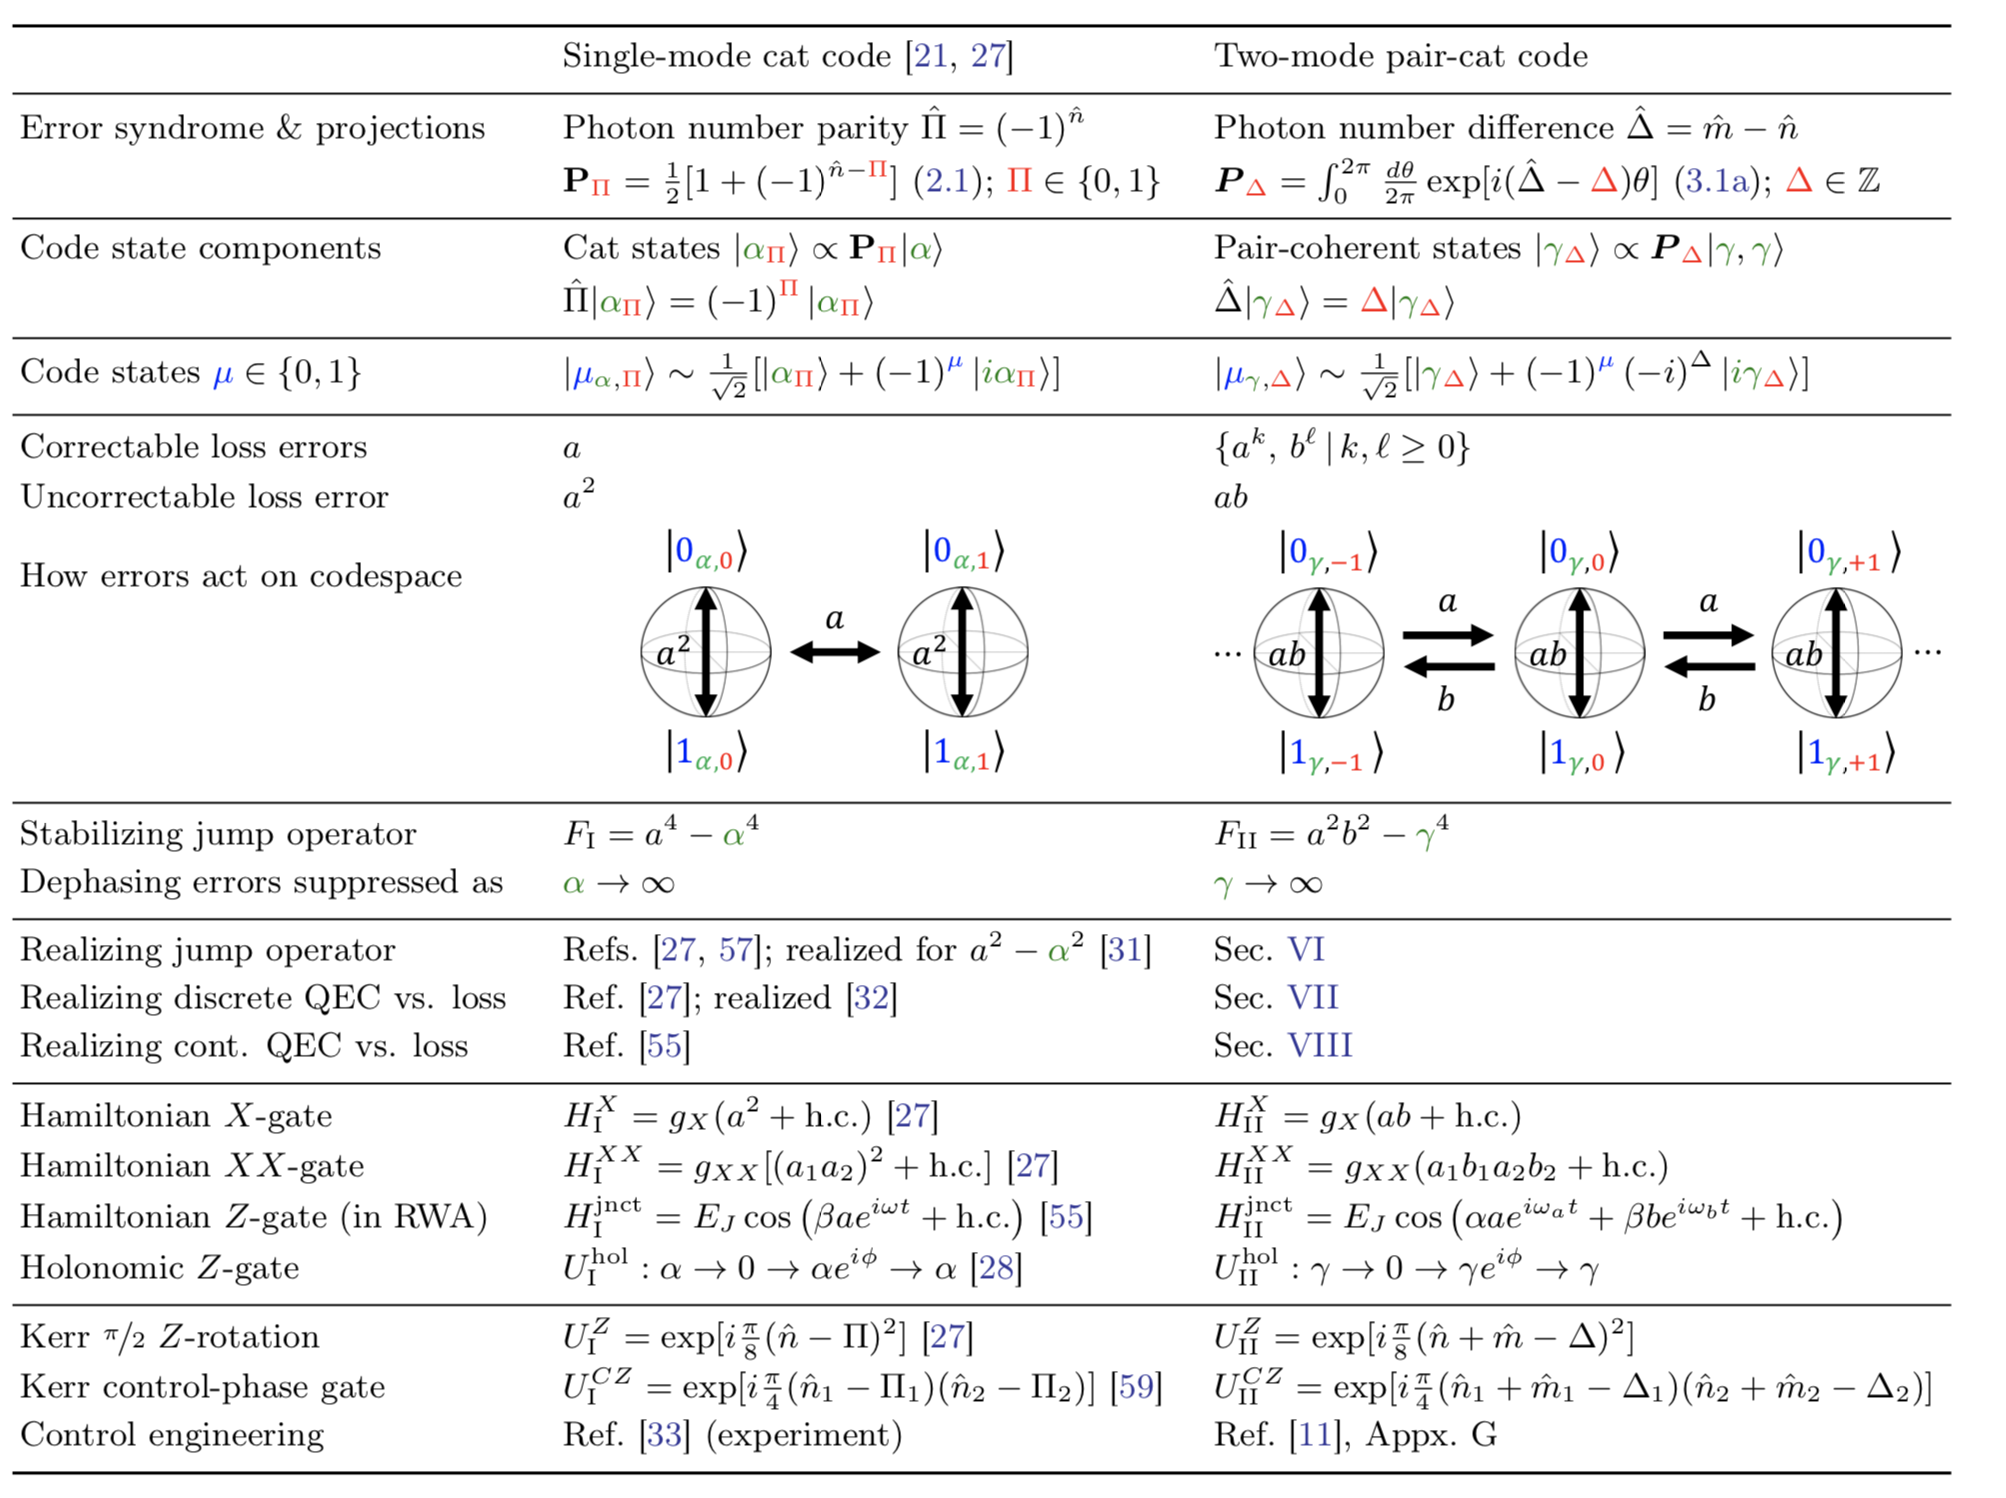
\includegraphics[width=\linewidth,keepaspectratio]{pair_cat.png}	
\caption{Figure from \cite{albert2018multimode} comparing single-mode cat codes to pair-cat codes}
\end{figure}


\subsubsection{Binomial Codes}
\label{sec:multi-binom}
\subsubsection*{$\chi^{(2)}$ Binomial Code}

Cat codes’ universal gate set relies on induced four-wave mixing interactions in Josephson junctions, which are much stronger than optical four-wave mixing in Kerr media. Cat codes have lower encod- ing overhead than generic QEC codes, because they introduce fewer error mechanisms. In addition, their requiring fewer physical resources than generic QEC codes makes it easier for them to reach the break-even point 

Quantum computation using only these resources is of interest because the χ(2) interaction is a lower-order nonlinearity, hence po- tentially stronger than four-wave mixing. Furthermore, excit- ing new technologies—such as solid-state circuits [24], flux- driven Josephson-junction parametric amplifiers [25–27], su- perconducting resonator arrays [28, 29], ring resonators [30], and frequency-degenerate double-lambda systems [31]—have been expanding the platforms for and increasing the efficien- cies of χ(2) interactions.

Unfortunately, the single-photon qubit basis used in Ref. [23] is not closed under χ(2) Hamiltonian evolutions, nor is it suitable for error correction, because any single-photon- loss error will destroy the quantum information carried by the qubit. Moreover, existing single-photon, multi-mode, QEC codes—such as the bosonic code [9], the quantum parity- check code [19], and the NOON code [34]—are not designed for hardware-efficient operation on an underlying architecture comprised of χ(2) interactions and linear optics.

In the present paper we take the next step, by proposing the first QEC codes for χ(2)-based universal quantum computa- tion and then demonstrating their hardware efficiency. To do so we establish a symmetry-operator framework, that lever- ages the symmetry of the physical subspace supporting the logical codewords and the symmetry of the measurable syn- dromes.


It is worth emphasizing that the χ(2) BC is the first Fock- basis bosonic QEC code that can correct N -photon-loss errors using O(N) photons for its encoding; all previous bosonic QEC codes with that error-correction capability require en- coding with O(N2) photons [9, 14, 16–19, 34, 37, 38]. Be- ing able to correct the loss of a constant fraction of the total photons for any code size is of great advantage for both large- scale quantum computation and long-range quantum commu- nication. However, the χ(2) BC requires channel-monitoring resources—which our other codes do not—that it uses to de- termine the number of photons that have been lost or gained. Our result thus highlights the importance of channel monitor- ing for the extra error-correction power it can provide by ob- viating a constraint from the error-correction condition [39], and it alerts us to the need for resource-efficient channel mon- itoring.

To verify that χ(2) BC’s satisfies the preceding error- correction condition. let us start with the simplest case, the N = 2 code in which each logical qubit is encoded as


This code uses a notion of "symmetry operators". First, we consider $N$-pump-photon 3-mode subspace $\mathcal{H}_N$ and observe that all states $\ket{\psi} = \sum_{n=0}^N c_n \ket{n, n, N-n} \in \mathcal{H}_N$ obey the following relations

\begin{align}
\begin{split}
	(\hat{n}_s + \hat{n}_p) \ket{\psi} &= N\ket{\psi} \\
	(\hat{n}_i + \hat{n}_p) \ket{\psi} &= N\ket{\psi} \\
	(\hat{n}_s - \hat{n}_i) \ket{\psi} &= 0\ket{\psi}
\end{split}
\end{align}

where $\hat{n}_k \equiv \hat{a}_k^\dag\hat{a}_k$ for each of the three modes $k = s, i, p$. Hence, the photon number parity vector

\begin{align*}
P &= [\hat{n}_s + \hat{n}_i, \hat{n}_s + \hat{n}_p, \hat{n_i + n_p}  ] \mod 2\\
&= [2N, N, N] \mod 2
\end{align*}

is constant $\forall \ket{\psi}$. Motivated by this, we can define symmetry operators 

\begin{align*}
\hat{Z}_{s, p}^{(N + 1)} = \exp(i 2 \pi / (N+1))	\hat{Z}_{s}^{(N + 1)} \otimes \hat{Z}_{p}^{(N + 1)} \\
\hat{Z}_{s, p}^{(N + 1)} = \exp(i 2 \pi / (N+1))	\hat{Z}_{s}^{(N + 1)} \otimes \hat{Z}_{p}^{(N + 1)}
\end{align*}

where

\begin{align*}
\hat{Z}_{k}^{(N + 1)} \equiv \sum_{n=0}^{N}\exp(i 2 \pi n / (N+1))	\ket{n}_k \bra{n}_k
\end{align*}

such that $\ket{n}_k, n \in 0, 1, \cdots, N$ is an $n$-photon Fock state of mode $k, k = s, i, p$.


In order to redundantly encode a lower-dimensional logical basis into a higher-dimensional physical basis, we need additional symmetry operators to stabilize the logical state: within the code’s physical subspace, only the simultaneous unity-eigenvalue eigenstates of all symmetry operators in the given set will be selected as logical-basis states.

In the case of the $\chi^{(2)}$ binomial code, one enforces the physical-subspace symmetry characterized by $\{ \hat{Z}_{s, p}^{(2N)}, \hat{Z}_{s, p}^{(2N)}\}$ above to restrict logical basis states to the subspace $\mathcal{H}_N$. Additionally, to leverage binomial symmetry that will protect the code subspace from distortion by photon loss or gain errors, we introduce the symmetry described by conjugating the photon-number inversion operator with the pseudo-beam-splitter operator. We will not detail this procedure and instead refer you to the original text \cite{niu2018hardware}.

The important aspect we wish to emphasize here is that this symmetry-operator formalism establishes a systematic framework for finding new QEC codes for available measurement schemes and physical subspace choices.

As an example, however, Niu et al show that when completing the set of symmetry operators, one finds that the simplest case is given by logical states

\begin{align*}
	\ket{B_{\uparrow}} &\sim \ket{0, 0, 3} + \sqrt{3}\ket{2, 2, 1}\\
	\ket{B_{\downarrow}} &\sim \ket{3, 3, 0} + \sqrt{3}\ket{1, 1, 2}
\end{align*}

and one can verify using (\ref{eq:k-l}) that the code is robust against up to second order loss or gain and first order dephasing across all modes.

Hardware Efficient Constructions

Noon codes

\begin{itemize}
	\item To create more useful quantum superpositions of Fock states which can store quantum information, it is necessary to couple the bosonic mode to a non-linear element, e.g., a superconducting qubit, a trapped ion, or a Rydberg atom
		\item $\chi(2)$ code uses $O(n)$ instead of $O(n^2)$ qubits that previous two mode codes had used to correct $m$ loss/gain/dephasing errors (Niu)
		\item Inspired by cat code, but uses lower order non-linearity
	\end{itemize}

\subsubsection{Importance of Bosonic Systems}

The first one is fundamental: with each added qubit, several new decoherence channels are added. This multiplies the number of possible errors and requires measuring more error syndromes. The second is practical: it still seems extremely challenging to build a register of more than on the order of 10 qubits.

\subsubsection{Future Developments}

apply performance methods to multi-mode codes

Notably, our symmetry- operator framework provides a systematic way for construct- ing bosonic QEC codes based on properties of the underlying system dynamics. It also provides a straightforward general- ization from qubit-basis three-mode encoding to qudit-basis multi-mode encoding.

\nocite{*}
\bibliography{qec_final_project.bib}
\bibliographystyle{amsplain}

\end{document}